% ----------------------------------------------------------
% Modelo ABNT para artigo científico (ABNT NBR 6022 / 10520)
% Compatível com arquivos .bib (Better BibLaTeX)
% ----------------------------------------------------------
\documentclass[12pt,oneside]{article}
% \documentclass[12pt,oneside]{abntex2}
% --- Pacotes básicos ---
\usepackage[english,brazilian]{babel}
\usepackage[utf8]{inputenc}
\usepackage[T1]{fontenc}
\usepackage{graphicx,url}
\usepackage{setspace}
\usepackage{enumitem}
% \usepackage{caption}
\usepackage[section]{placeins}  % impede figuras fora da seção

% --- Bibliografia ABNT ---
\usepackage{csquotes}
\usepackage[style=abnt,backend=biber,language=brazil]{biblatex}
\addbibresource{DR_Estudo.bib}      % ln -s /Users/daltonreis/GitHub/disciplinas/UDESC_2025/Dr/DR_Estudo.bib

% --- Ajustes de espaçamento e margens ---
\usepackage[a4paper,margin=2.5cm]{geometry}
% \setstretch{1.5}
\sloppy

% --- Formatar textos de código ---
% \lstlistoflistings        % colocar no texto para gerar uma lista desses itens
\newcommand{\code}[1]{\texttt{#1}}
\usepackage{listings}
\lstset{
  basicstyle=\ttfamily,      % monoespaçada
  columns=fullflexible,      % melhor espaçamento
  keepspaces=true,           % preserva espaços
  upquote=true               % aspas retas em verbatim
}
\renewcommand{\lstlistingname}{Listagem}
\renewcommand{\lstlistlistingname}{Lista de listagens}

\newenvironment{resumoEng}{%
  \par\vspace{1em}%
  \begin{center}\bfseries Abstract\end{center}%
  \begin{quotation}%
}{\end{quotation}}

\newenvironment{resumoPort}{%
  \par\vspace{1em}%
  \begin{center}\bfseries Resumo\end{center}%
  \begin{quotation}%
}{\end{quotation}}

% --- Formatação de título ---
\title{Título do Artigo Segundo as Normas da ABNT}
\author{Autor(a) Nome Completo\thanks{Instituição, e-mail: autor@exemplo.com}}
\date{2025}

\begin{document}
\maketitle

\begin{otherlanguage*}{english}
\begin{resumoEng}
This is the abstract in English. It should succinctly present the article’s
objective, method, results, and conclusions.

\textbf{Keywords:} Augmented Reality, Education, Learning.
\end{resumoEng}
\end{otherlanguage*}

\begin{resumoPort}
Este é o resumo em língua portuguesa. Deve conter uma síntese clara do conteúdo,
incluindo objetivo, método, resultados e conclusões.

\textbf{Palavras-chave:} Realidade Aumentada, Educação, Aprendizagem.
\end{resumoPort}

% ----------------------------------------------------------
% Dicas
% 	•	\input{arquivo} não insere quebra de página e é ideal para seções pequenas.
% 	•	\include{arquivo} insere quebra de página antes e depois, e gera arquivos .aux individuais (bom para projetos grandes).

% ----------------------------------------------------------

% ----------------------------------------------------------
\section{Introdução}\label{sec:introducao}

A introdução apresenta o tema, contextualização, problema e objetivo.  

% Exemplo de citação parentética \cite{albuquerqueToyUserInterfaces2021}.  
Exemplo de citação parentética \parencite{albuquerqueToyUserInterfaces2021}.  

Exemplo de citação narrativa, que segundo
\textcite{aragaoEnsinoProgramacaoPensamento2023}, os jogos sérios podem aumentar
o engajamento.

Exemplo de citação com página
\cite[p.~25]{azumaRecentAdvancesAugmentedReality2001}:
\begin{displayquote}
\small
Com um texto para citação direta que deve ter mais de três linhas de texto
falando sobre alguma coisa qualquer. Assim se tem três linhas de um texto
qualquer, pois se precisa ter todo esse texto.
\end{displayquote}


% ----------------------------------------------------------
\section{Referencial Teórico}\label{sec:referencialTeorico}

De acordo com \cite{pimentelDesignScienceResearch2020}, a pesquisa baseada em
design oferece um processo iterativo de melhoria de artefatos educacionais
(\ref{sec:apendiceA}).


% ----------------------------------------------------------
\section{Metodologia}\label{sec:metodologia}

Descreve o método, instrumentos e procedimentos adotados.  
Use listas com \texttt{enumitem}:
\begin{enumerate}[label=\alph*), itemsep=0pt, topsep=0pt, parsep=0pt, partopsep=0pt]
  \item definição das variáveis;
  \item aplicação dos testes;
  \item análise dos resultados.
\end{enumerate}


% ----------------------------------------------------------
\section{Resultados e Discussão}\label{sec:resultadosDiscussao}

Os resultados devem ser apresentados de forma objetiva, com tabelas e figuras
(Figura~\ref{fig:exemplo}).

\begin{figure}[ht]
\centering
\caption{Exemplo ilustrativo de figura}
\begingroup
\setlength{\fboxsep}{0pt}
\fbox{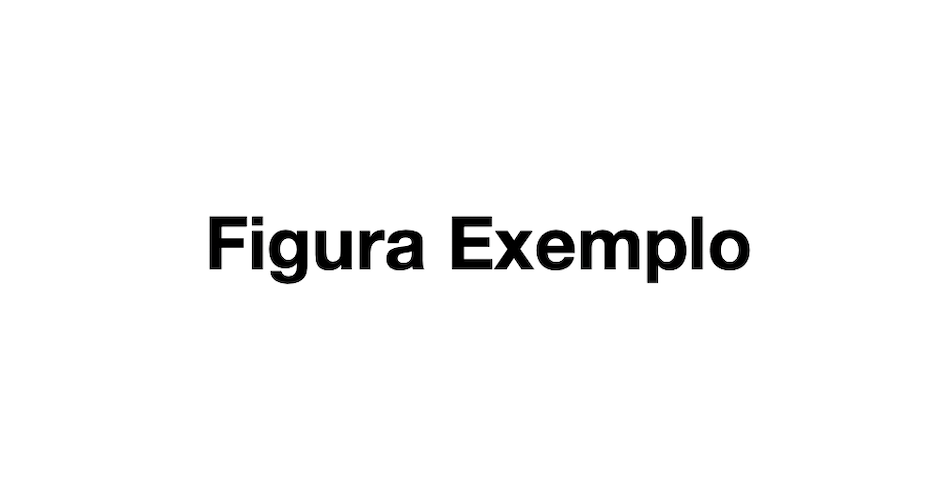
\includegraphics[width=0.7\textwidth]{figura.png}}
\endgroup
\\[2pt]
{\small Fonte: elaborado pelo autor.}
\label{fig:exemplo}
\end{figure}
\vspace{-6pt}


% ----------------------------------------------------------
\section{Considerações Finais}\label{sec:consideracoesFinais}

As conclusões devem relacionar os resultados aos objetivos. 

Exemplo para ser usado com tiver trecho de código, como exemplo o nome de uma
classe \texttt{Algoritmo}.

Ou ainda, método \verb|push_back| da classe \texttt{Vector}. Use texttt\ para
palavras/identificadores e verb quando houver barras, sublinhados, etc.

A classe \code{Algorithm} gerencia a lista de \code{logs}.

A classe \lstinline!Algorithm! valida os blocos.

\begin{lstlisting}[language=Java, caption={Exemplo de classe}, label={lst:ex}]
class Algorithm { ... }
\end{lstlisting}


% ----------------------------------------------------------
\printbibliography

% ----------------------------------------------------------
\appendix
\renewcommand{\thesection}{Apêndice \Alph{section}}

\end{document}